\chapter[Conclusions and Future Work]{Conclusions and Future Work}
\label{chap:Conclusions}

Research presented in this dissertation addresses the problem of how regular users can manage autonomy by managing information at different scale and hierarchy. This automy management approach is applied to the application domain of using a UAV to support Wilderness Search and Rescue. Autonomous components and autnonomy management tools are designed at three distinctive scales, \textbf{Strategic}, \textbf{Between-Episodes}, and \textbf{Within-Episode}, following the autonomy integration guidelines we identified. And by managing two information representations, a \textit{probability distribution map} and a \textit{task-difficulty map}, at each scale, the domain expert user becomes an ``intelligent sersor'' and can feed information to each autonomous component in a form the autonomous component can understand. Doing so enables the user to influence the behavior of the autonomous subsystem without understanding the statistical models or complex algorithms used in the autonomous components.

%=====================================================================================================
\section{Conclusions}
\label{conclusions}




%=====================================================================================================
\section{Contributions}
\label{contributions}

This dissertation has the following main contributions to Computer Science research.

\begin{itemize}
\item We identified autonomy integration challenges along two dimensions: \textit{attributes of an intelligent system} (capability, information management, performance evaluation) and \textit{scale} (individual, collaborative agents, distributed system). These requirements served as a guideline in our design of the autonomous components and autonomy management tools in our proposed solution.
\item We propose a new autonomy management approach: managing autonomy by hierarchically managing information at three scales through two information representations: a \textit{probability distribution map} and a \textit{task-difficulty map}. We developed various autonomous components and autonomy management tools at each scale and demonstrated the usefulness of the approach.
\item We designed a Bayesian model that uses terrain features and past human behavior data to model lost-person behaviors. The user can influence the probability distribution map generated by changing prior beliefs and by selecting what subset of past human behavior data to feed to the model.
\item We designed two autonomy management tools that enable the user to manage the \textit{probability distribution map} and \textit{task-difficulty map} by mouse and finger gestures.
\item We proposed a heuristic, \textit{Mode Goodness Ratio}, which uses a Gaussian Mixture Model to prioritize search subregions, and enables a hierarchically search for effective paths through the parameter space at different levels of resolution.
\item We designed multiple path planning algorithms that support partial detection. We evaluated the performance of these algorithms against state-of-the-art algorithms using three real WiSAR scenarios and show that our algorithms generate near-optimal paths in real-time.
\item We proposed the Sliding Autonomy Interface that enables the user to manage path planning autonomy along two dimensions: constraints (spatial) and flight duration (temporal). Data from a user study show that this approach enables the human-automation team to outperform human or automation working alone, reduces the human's cognitive workload, and improves the human experience in the human-automation. interaction.
\end{itemize}

%=====================================================================================================
\section{Future Work}
\label{futurework}

This section presents a few of the natural exptensions from current research that can be pursued as future work. We list them in the order of the three scales and show how they relate to the various components of the dissertation work.

\begin{figure}
\centering
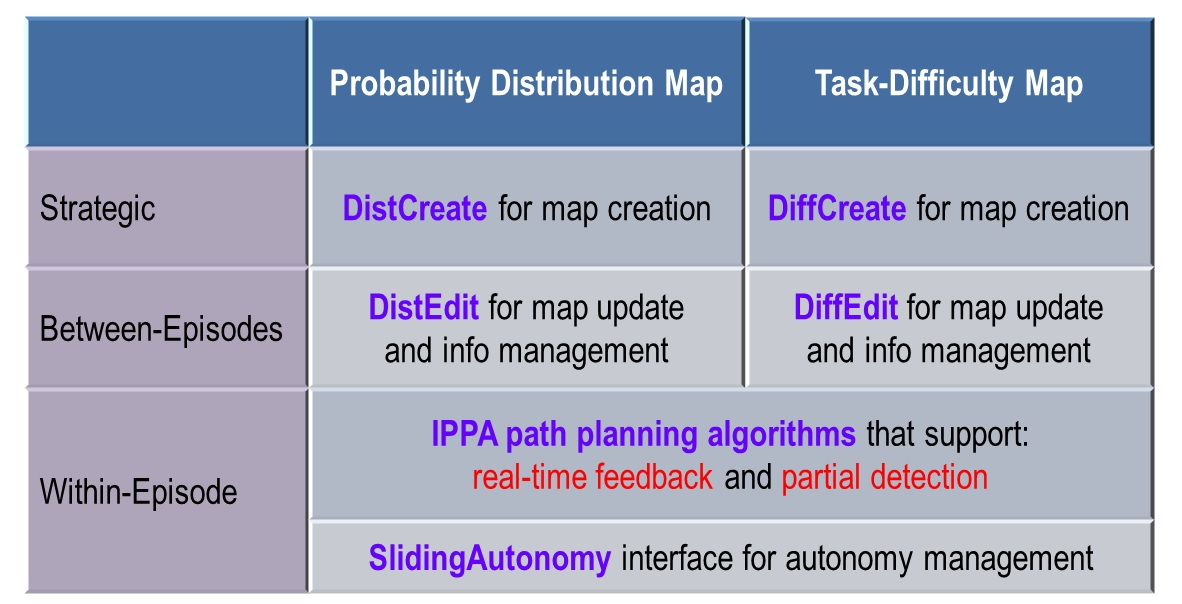
\includegraphics[width=6in]{ProjectComponents.JPG}
\caption{Autonomous components and autonomy management tools of the dissertation work at each scale/hierarchy.}
\label{ProjectComponents2}
\end{figure}

%===================================================
\subsection{At the Strategic Scale}

After the searcher provides some initial lost person profile information (such as age, gender, etc.), the system will suggest transitional probability values based on statistics from past incidents~\cite{Koester2008Lost}. The searcher can use the suggested parameters or specify them manually using the proposed information management tool, \textbf{ParamMod}. Figure~\ref{Mockup1} shows a mock up screen of the \textbf{ParamMod} tool. A searcher can move two sliders to set the mean and standard deviation of a Beta distribution and see immediately how the shape of the Beta distribution would change respectively. We use mean and standard deviation parameters because they are easy to understand (in contrast to the $\alpha$ and $\beta$ parameters in the Beta distribution function). As the searcher changes the shape of each transitional probability distribution, the searcher will also see immediately how the changes affect the final 3D probability distribution map. This immediate visual feedback allows the user to understand causal effects and therefore helps the user form a mental model of the system that is similar to how the system truly works. Computationally, instant feedback requires that we perform matrix computations on the GPU using CUDA (Compute Unified Device Architecture) architecture. We have been collaborating with Mike Roscheck to implement this and will publish a paper on it.

\begin{figure}
\centering
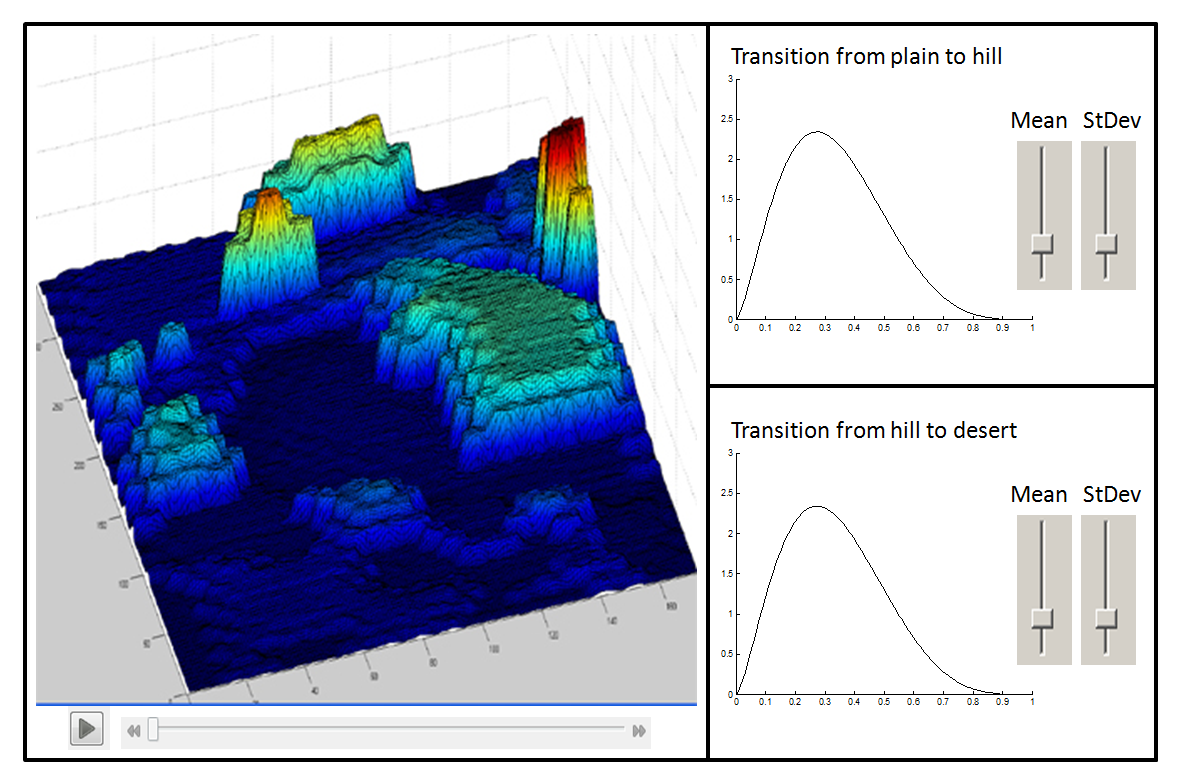
\includegraphics[width=3in]{Mockup1.png}
\caption{A mock up screen for the management tool interface at the general trend scale.}
\label{Mockup1}
\end{figure}

Comparing the prior predictive to the posterior predictive distribution should allow the searcher to understand the causal relationship of how the decision affects the probability distribution map produced. We plan to use selected geocacher GPS track logs downloaded from Everytrail.com as the dataset. We will also create utility tools to process these GPS track logs, including automatically downloading and labeling related terrain features.


%The current Bayesian model uses external calls to MATLAB for large-size matrix multiplications and it takes roughly 4 seconds to multiple two 608 $\times$ 608 matrices. Since one matrix multiplication is needed for each time interval (1 minute), generating a predictive probability distribution for a 3-hour duration would require 180 matrix multiplications, which will take 12 minutes computation time. If after a user changes a model parameter, he/she has to wait 12 minutes to see how the parameter change affects the final product of the model, it is not very useful especially with respect to seeing the causal relationship. We propose to take advantage of powerful GPUs and use the CUDA (Compute Unified Device Architecture) parallel computation architecture developed by NVIDIA to speed up the matrix multiplications. Initial test runs of multiplying two 608 $\times$ 608 matrices on a GeForce GTX480 GPU took only 2 miliseconds. Such speed up enables the user to see immediately how parameter changes could affect the shape of the 3D probability distribution produced by the model. However, the immediate feedback is only avaible when computing the prior preditive probability (without using past human behavior data) because computing the posteriors of the transitional probabilities still takes 220 seconds when using the MCMC algorithm.


%Because intended destination and trail-following behaviors are important factors that can affect a lost person's behavior~\cite{Lin2010Bayesian}, we plan to include them in our \textbf{TBMod} model. Because trail data are not readily available directly from public resources, our utility tools will allow a user to trace trails from an overlaid satellite image of the region and add the topographical feature to the dataset. To add the intended destination feature, we include a prior node in our Bayesian network representing the probability of traveling to different directions with respect to how dispersed the direction is from the intended destination. This prior node will follow a categorical distribution, but the probability of each category is determined by a Gaussian distribution. A scaler parameter $s$ will be used to specify how the Gaussian distribution can be divided into different categories.

%The autonomy interface management tool should allow the searcher to first mark Point Last Seen and intended destination on the terrain map overlay, then specify lost person profile information such as age group and gender,  next choose whether to use past human behavior data, and finally choose whether to specify transitional probabilities manually.

%===================================================
\subsection{At the Between-Episodes Scale}

%===================================================
\subsection{At the Within-Episode Scale}




